%!TEX root = ../Main.tex

% \pagebreak
\section{Core language}
\label{s:core}

%!TEX root = ../Main.tex
\begin{figure}
  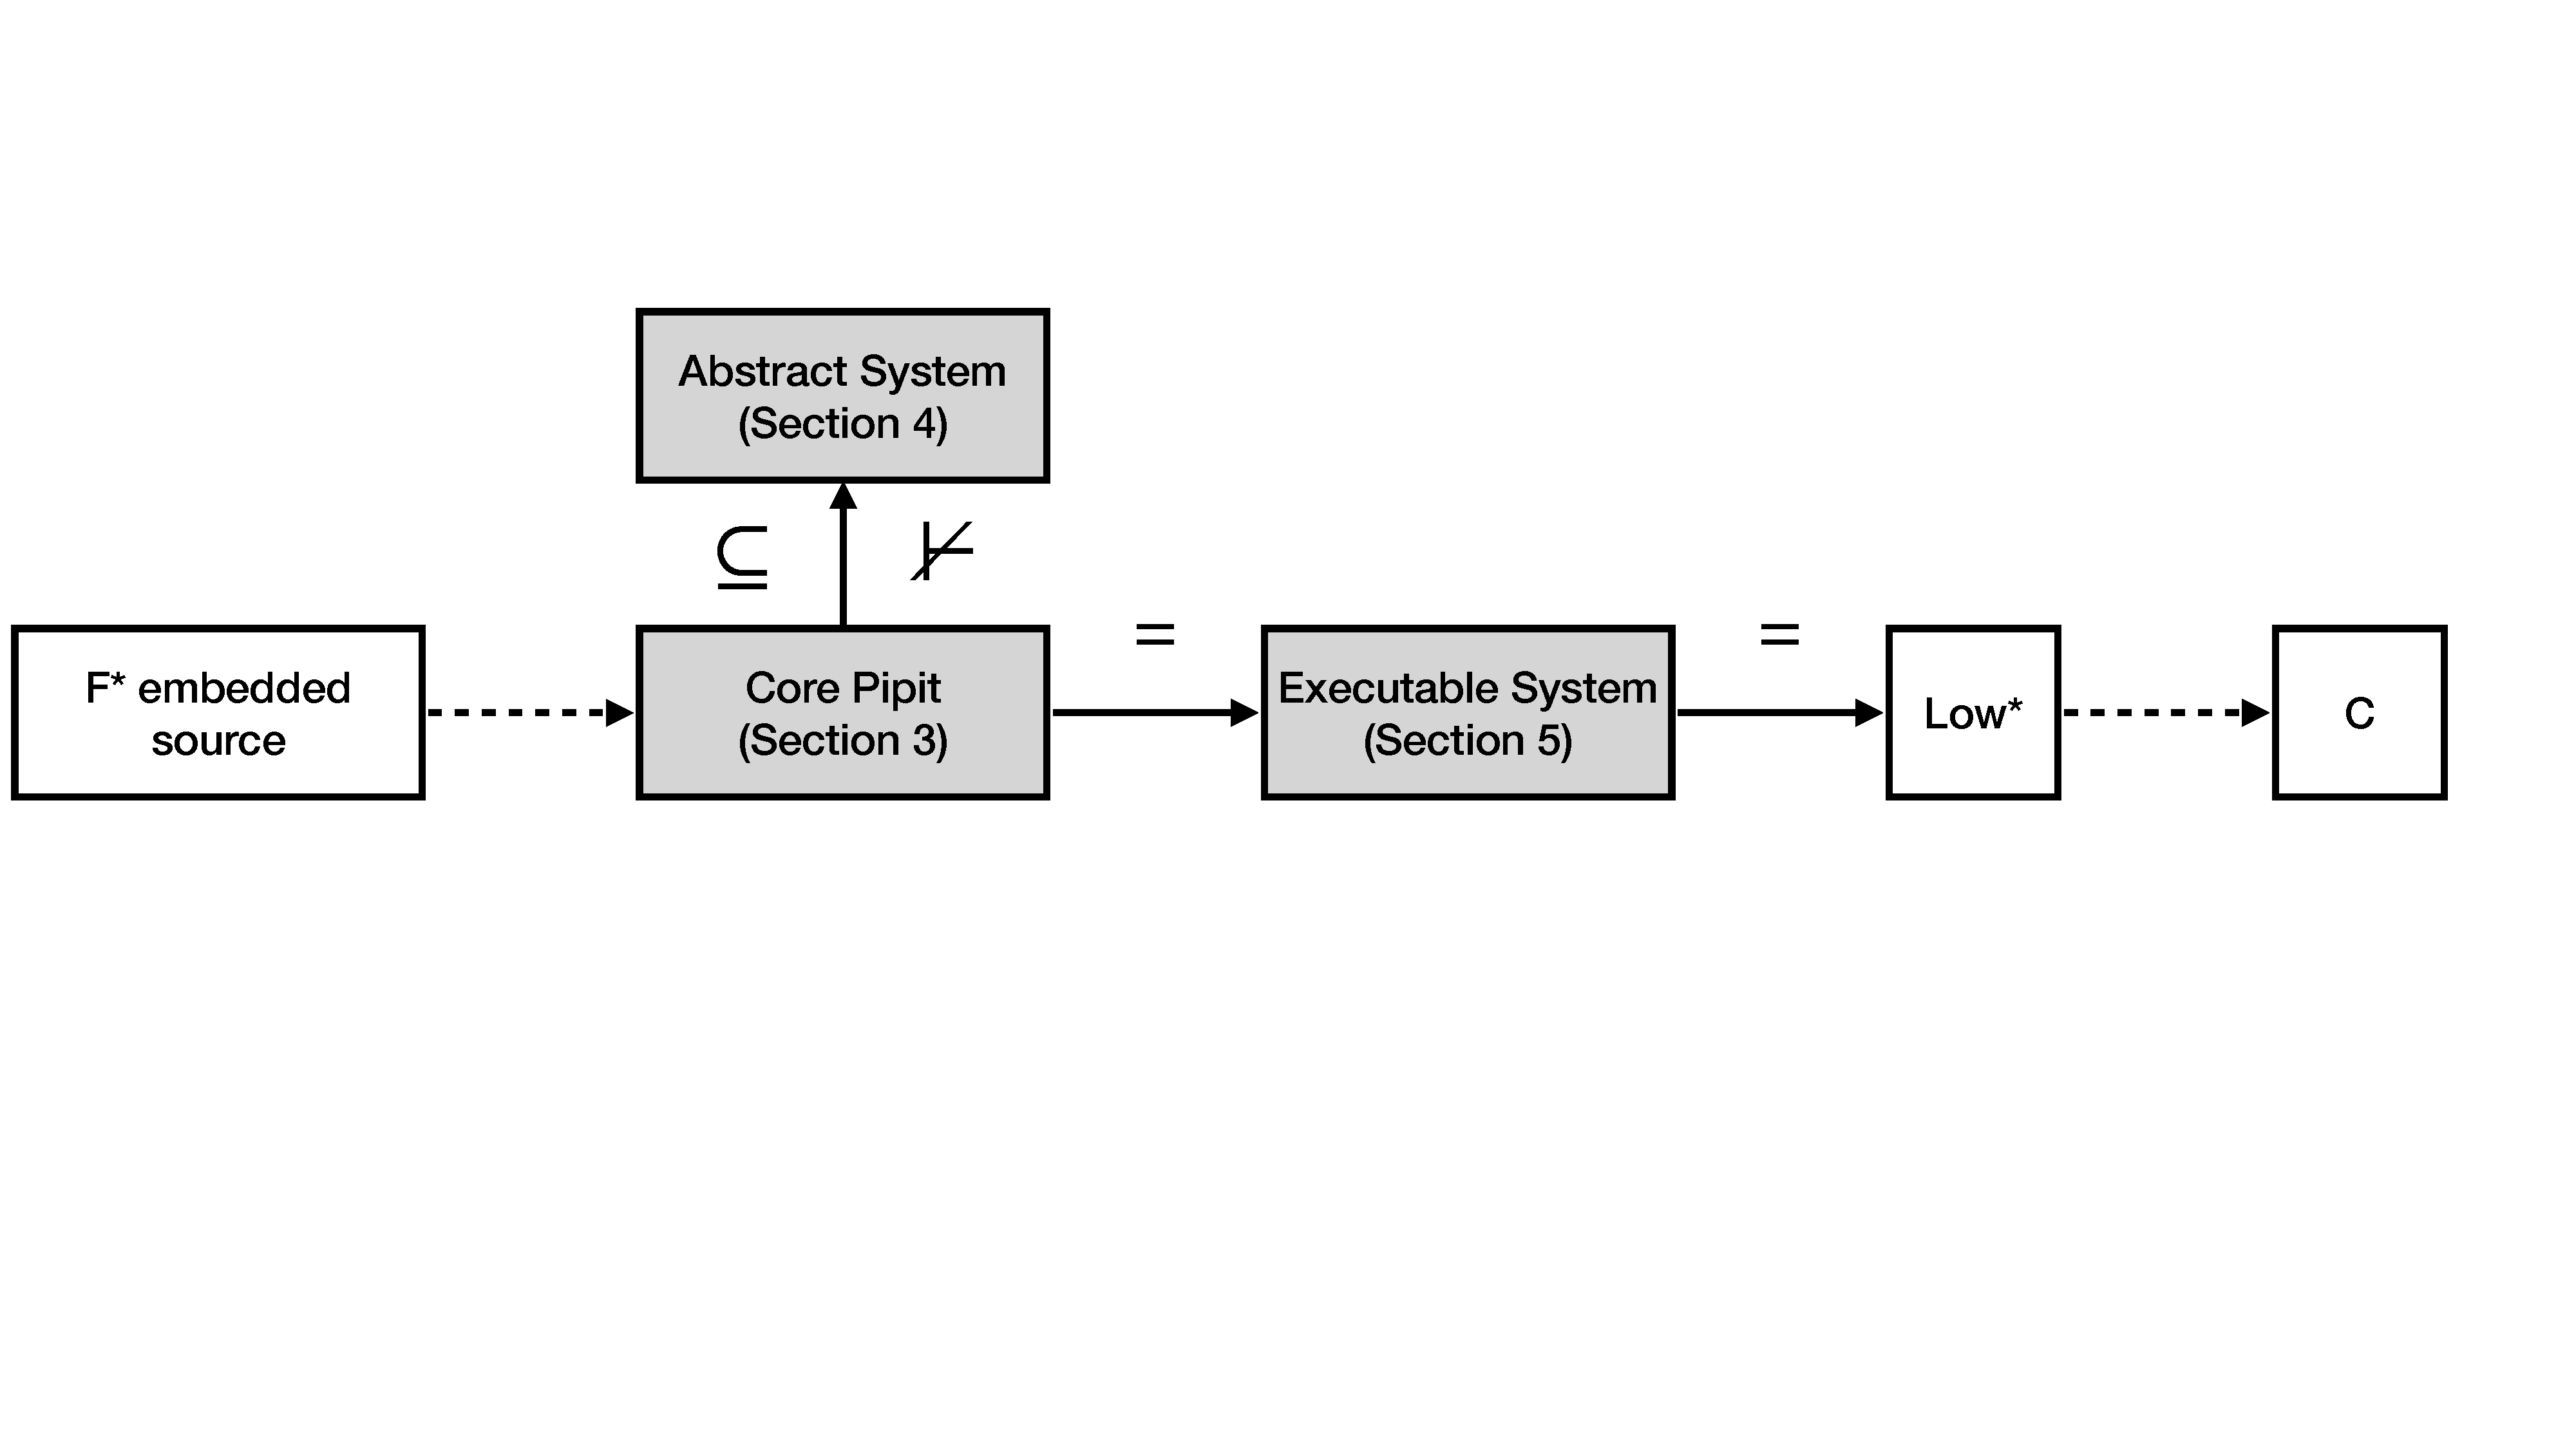
\includegraphics[width=\textwidth]{figures/core-structure.pdf}
\caption{Architecture of Pipit. The gray boxes and solid arrows are defined in this paper. The white boxes and dashed arrows are trusted components. The labels next to the arrows denote properties of the translation. The refinement label ($\subseteq$) indicates a verified abstraction relation; the negated entailment ($\not\vdash$) indicates that the entailment relation --- contracts and checked properties proven on abstract system apply to the checked semantics --- is not yet verified; the equivalence ($=$) denotes a verified equivalence relation.}
\label{f:core:structure}
\end{figure}


We now introduce the core Pipit language.
Note that this form differs slightly from the surface syntax presented earlier in \autoref{s:motivation}, which used the syntax of the metalanguage \fstar{}, as well as including proofs in \fstar{} itself.


\autoref{f:core:structure} shows the architecture of Pipit.
On the left-hand-side, the surface syntax embedded in \fstar{} is shown; this includes some Pipit-specific syntactic sugar.
The translation from the surface syntax to the core language is trusted.
There are two targets from the core language: abstract transition systems for verification, and executable transition systems for extraction to C.
The translation from the abstract systems is verified to be an abstraction according to the dynamic semantics (\autoref{s:core:dynamic}).
One property that still remains to be proven is that if the abstract transition system says a contract or checked property holds, then the same contract or property holds on the original semantics; this is denoted as negated entailment in the figure ($\not\vdash$).
The translation to executable transition system is proven to be semantics preserving, as is the subsequent translation to \lowstar{}.
The translation from \lowstar{} to C is external to this paper and forms part of our trusted computing base.


\autoref{f:core-grammar} defines the grammar of Pipit.
The expression form $e$ includes standard syntax for values ($v$), variables ($x$) and primitive applications ($p(\ov{e})$).
Most of the expression forms were introduced informally in \autoref{s:motivation} and correspond to the clock-free expressions of Lustre~\cite{caspi1995functional}.

%!TEX root = ../Main.tex

\begin{figure}
  \[
  \begin{array}{lrlr}
    e, e' & := & v ~|~ x ~|~ p(\ov{e}) & \mbox{(values, variables and operations)} \\
          & | & \xfby{v}{e} ~|~ \xrec{x}{e[x]} & \mbox{(followed-by (delay) and recursive streams)} \\ % & | & \xthen{e}{e'} \\
          & | & \xlet{x}{e}{e'[x]} & \mbox{(let-expressions)}\\
          & | & \xcheckP{\PStatus}{e_{\text{prop}}} & \mbox{(checked properties)} \\
          & | & \xcontractP{\PStatus}{\erely}{\eimpl}{x\!.~\eguar} & \mbox{(rely-guarantee contracts)} \\
          % & | & \xcheck{e} \\
    \\
    v & := & n \in \mathbb{N} ~|~ b \in \mathbb{B} ~|~ r \in \mathbb{R} ~|~ \hdots  & \mbox{(values)} \\
    p & := & (+) ~|~ (-) ~|~ (\times) ~|~ @if-then-else@ ~|~ \hdots & \mbox{(primitives)} \\
    \\
    \PStatus & := & \PSValid ~|~ \PSUnknown & \mbox{(property statuses: valid or unknown)}\\
    \\
    \sigma & := & \sgl{\ov{x \mapsto v}} & \mbox{(heaps)} \\
    \Sigma & := & \sigma ~|~ \Sigma;\sigma & \mbox{(streaming history environments)} \\
    %   \\
    \tau, \tau' & := & \mathbb{N} ~|~ \mathbb{B} ~|~ \tau \times \tau ~|~ \hdots & \mbox{(value types)} \\
    \Gamma & := & \cdot ~|~ x : \tau, \Gamma & \mbox{(type environments)}  \\
    \end{array}
  \]
  \caption{Pipit core language grammar, which contains expressions $e$, values $v$, primitive operations $p$, and property statuses $\PStatus$.}
  \label{f:core-grammar}
\end{figure}

The expression syntax for delayed streams ($\xfby{v}{e}$) denotes the previous value of the stream $e$, with an initial value of $v$ when there is no previous value.
% Streams can also be composed together using the \emph{then} notation ($\xthen{e}{e'}$) which denotes that the value of stream $e$ is used for the first step, followed by the values from stream $e'$ for subsequent steps.

Recursive streams, which can refer to previous values of the stream itself, are defined using the fixpoint operator ($\xrec{x}{e[x]}$); the syntax $e[x]$ means that the variable $x$ can occur in $e$.
% To ensure that streams are productive,
As in Lustre, recursive streams can only refer to their previous values and must be \emph{guarded} by a delay: the stream $(\xrec{x}{\xfby{0}{(x + 1)}})$ is well-defined, but stream $(\xrec{x}{x + 1})$ is invalid and has no computational interpretation.
This form of recursion differs slightly from standard Lustre, which uses a set of mutually-recursive bindings.
% We use this form to define a substitution-based operational semantics that is syntax-directed, as opposed to the mutually-recursive form in \cite{caspi1995functional} which is not syntax-directed.
% Our semantics has a simpler proof of determinism; we believe it has simplified other necessary proofs too and will perform further evaluation.
Although we cannot express mutually-recursive bindings in the core syntax here, we can express them as a notation on the surface syntax by combining the bindings together into a single tuple.

Checked properties and contracts are annotated with their property status $\PStatus$, which can either be valid ($\PSValid$) or unknown ($\PSUnknown$).
For checked properies $\xcheckP{\PStatus}{e}$, the property status denotes whether the property has been proved to be valid.

Contracts $\xcontractP{\PStatus}{\erely}{\ebody}{\rawbind{x}\eguar[x]}$ involve two verification conditions.
Firstly, when a contract is \emph{defined}, the definer must prove that the body $\ebody$ satisfies the contract: roughly, if $\erely$ is always true, then $\eguar[x := \ebody]$ is always true.
Secondly, when a contract is \emph{instantiated}, the caller must prove that the environment satisfies the precondition: that is, $\erely$ is always true.
Conceptually, then, a contract could have two property statuses: one for the definer, and one for the instantiation.
However, in practice, it is not useful to defer the proof of a contract definition --- one could achieve a similar effect by replacing the contract with its implementation.
For this reason, we only annotate contracts with one property status, which denotes whether the instantiation has been proved to satisfy the precondition.

For the presentation of the formal grammar here, we consider only a fixed set of values and primitives; in practice, the implementation is parameterised by a primitive table which we extend with immutable array operations for the TTCAN driver logic in \autoref{s:evaluation}.

Streams $V$ are represented as a sequence of values; streaming history environments $\Sigma$ are streams of heaps.
Types $\tau$ and type environments $\Gamma$ are standard.

\begin{figure}
  \[
    \boxed{\typing{\Gamma}{e}{\tau}}
    \quad
    \boxed{\mtyping{}{v}{\tau}}
  \]

  \[
    \ruleIN{
      \mtyping{}{v}{\tau}
    }{
      \typing{\Gamma}{v}{\tau}
    }{TValue}
    \quad
    \ruleAx{\typing{\Gamma}{x}{\Gamma(v)}}{TVar}
  \]

  \[
    \ruleIN{
      \typing{\Gamma}{e}{\tau \to \tau'}
      \qquad
      \typing{\Gamma}{e'}{\tau}
    }{\typing{\Gamma}{e~e'}{\tau'}}{TApp}
  \]

  \[
    \ruleIN{
      \typing{\Gamma}{v}{\tau}
      \qquad
      \typing{\Gamma}{e'}{\tau}
    }{
      \typing{\Gamma}{\xfby{v}{e'}}{\tau}
    }{TFby}
  \]

  \[
    \ruleIN{
      \typing{\Gamma}{e}{\tau}
      \qquad
      \typing{\Gamma}{e'}{\tau}
    }{\typing{\Gamma}{\xthen{e}{e'}}{\tau}}{TThen}
  \]

  \[
    \ruleIN{
      \typing{x : \tau, \Gamma}{e}{\tau}
    }{
      \typing{\Gamma}{\xrec{x}{e[x]}}{\tau}
    }{TRec}
  \]

  \[
    \ruleIN{
      \typing{\Gamma}{e}{\tau}
      \qquad
      \typing{x : \tau, \Gamma}{e'}{\tau'}
    }{
      \typing{\Gamma}{\xlet{x}{e}{e'[x]}}{\tau'}
    }{TLet}
  \]

  \[
    \ruleIN{
      \typing{\Gamma}{e}{\mathbb{B}}
    }{
      \typing{\Gamma}{\xcheck{e}}{\tt{unit}}
    }{TCheck}
  \]

  \caption{Typing rules for Pipit defined in terms of two judgment forms: $\typing{\Gamma}{e}{\tau}$ denotes that expression $e$ describes a \emph{stream} of values of type $\tau$; and $\mtyping{}{v}{\tau}$, which denotes that closed meta-value $v$ has type $\tau$ and is not defined here.}\label{f:core-typing}
\end{figure}

We define the typing judgments for Pipit in \autoref{f:core-typing}.
Most of the typing rules are standard for an unclocked Lustre.
The typing judgment $\typing{\Gamma}{e}{\tau}$ denotes that, in an environment of streams $\Gamma$, expression $e$ denotes a stream of type $\tau$.
This core typing judgment differs from the surface syntax used in \autoref{s:motivation}, which used an explicit stream type; for the core language, we instead assume that everything is a stream.

For values, we use an auxiliary judgment form $\mtypingval{v}{\tau}$ to denote that value $v$ has type $\tau$.
Likewise, for primitives we use the auxiliary judgment form $\mtypingprim{p}{(\tau_1 \times \cdots \hdots \times \tau_n) \to \tau'}$ to denote that primitive $p$ takes arguments of type $\tau_i$ and returns a result of type $\tau'$.
Primitives are pure, non-streaming functions.

Rules \textsc{TValue}, \textsc{TVar}, \textsc{TPrim} and \textsc{TLet} are standard.

Rule \textsc{TFby} states that expression $\xfby{v}{e}$ requires both $v$ and $e$ to have equal types; the result is the same type.

Rule \textsc{TRec} states that a recursive stream $\xrec{x}{e}$ has the recursive stream bound inside $e$.
The recursion must also be guarded, in that any recursive references to $x$ are delayed, but this requirement is performed as a separate syntactic check described in \autoref{s:core:causality}.

Rule \textsc{TCheck} states that statically checking a property $\xcheckP{\PStatus}{e}$ requires a boolean property $e$ and returns unit.

Finally, rule \textsc{TContract} applies for a contract $\xcontractP{\PStatus}{\erely}{\ebody}{\rawbind{x}\eguar[x]}$ with a body expression of some type $\tau$.
The overall expression has result type $\tau$.
Both rely and guarantee clauses must be boolean expressions.
Additionally, the guarantee clause can refer to the result value by $x$.

\subsection{Dynamic semantics}
\label{s:core:dynamic}
\begin{figure}
  \[ \boxed{\bigstep{\Sigma}{e}{v}} \]

  \[
    \ruleAx{\bigstep{\Sigma}{v}{v}}{Value}
    \quad
    \ruleAx{\bigstep{\Sigma_\bot; \sigma}{x}{\sigma(v)}}{Var}
  \]

  \[
    \ruleIN{
      \bigstep{\Sigma}{e}{(\mlamX)}
      \qquad
      \bigstep{\Sigma}{e'}{v'}
    }{\bigstep{\Sigma}{e~e'}{(\mlamX)~v'}}{App-Meta}
  \]

  % \[
  %   \ruleIN{\bigstep{\Sigma}{e}{v}}{\bigstep{\Sigma; \sigma}{\xpre{e}}{v}}{Pre}
  % \]

  \[
    \ruleAx{\bigstep{\sigma}{\xfby{v}{e'}}{v}}{$\mbox{Fby}_1$}
    \quad
    \ruleIN{\bigstep{\Sigma}{e'}{v'}}{\bigstep{\Sigma; \sigma}{\xfby{v}{e'}}{v'}}{$\mbox{Fby}_S$}
  \]

  \[
    \ruleIN{\bigstep{\sigma}{e}{v}}{\bigstep{\sigma}{\xthen{e}{e'}}{v}}{$\xthenarrow_1$}
    \quad
    \ruleIN{\bigstep{\Sigma}{e'}{v'}}{\bigstep{\Sigma; \sigma}{\xthen{e}{e'}}{v'}}{$\xthenarrow_S$}
  \]

  \[
    \ruleIN{
      \bigstep{\Sigma}{e[x := \xrec{x}{e}]}{v}
    }{
      \bigstep{\Sigma}{\xrec{x}{e[x]}}{v}
    }{Rec}
  \]

  \[
    \ruleIN{
      \bigstep{\Sigma}{e'[x := e]}{v}
    }{
      \bigstep{\Sigma}{\xlet{x}{e}{e'[x]}}{v}
    }{Let}
  \]

  \[
    \ruleIN{
      \bigstep{\Sigma}{e}{\top}
    }{
      \bigstep{\Sigma}{\xcheck{e}}{()}
    }{Check}
  \]

  \caption{Bigstep operational semantics for Pipit defined in terms of the judgment form $\bigstep{\Sigma}{e}{v}$; this judgment form denotes that evaluating expression $e$ under streaming history $\Sigma$ results in value $v$.}\label{f:core-bigstep}
\end{figure}

The dynamic semantics of Pipit are defined in \autoref{f:core-bigstep}.
We present our semantics in a big-step form.
This differs somewhat from traditional \emph{reactive} semantics of Lustre~\cite{caspi1995functional}.
Our big-step semantics emphasises the equational nature of Pipit, as it is substitution-based, while the reactive semantics emphasises the finite-state streaming execution of the system.
We use transition systems for reasoning about the finite-state execution (\autoref{s:transition}), which is fairly standard~\cite{brun2023equation,champion2016kind2,raymond2008synchronous}.
Previous work on the {\sc W-calculus}~\cite{gallego2021w} for linear digital signal processing filters makes a similar distinction and provides a non-streaming semantics for reasoning about programs and a streaming semantics for executing programs.


The judgment form $\bigstep{\Sigma}{e}{v}$ denotes that expression $e$ evaluates to value $v$ under streaming history $\Sigma$.
The streaming history is a stream of heaps; in practice, we only evaluate expressions with a non-empty streaming history.

Rule {\sc Value} states that evaluating a value results in the value itself.

Rule {\sc Var} states that to evalute a variable $x$ under some non-empty stream history $\Sigma; \sigma$, where $\sigma$ is the most recent heap, we look up the variable in $\sigma$.

Rule {\sc Prim} states that to evaluate a primitive $p$ applied to many arguments $e_1$ to $e_n$, we evaluate each argument separately; we then use the prim-sem metafunction to apply the primitive.

Rule $\textsc{Fby}_1$ evaluates a followed-by expression when the streaming history contains only a single element.
Here, $\xfby{v}{e}$ evaluates to $v$, as there is no previous value of $e$ to use.

Rule $\textsc{Fby}_S$ evaluates a followed-by expression when the streaming history contains multiple entries.
In this case, $\xfby{v}{e}$ proceeds to evaluate the previous value of $e$ by discarding the most recent entry from the streaming history.

Rule {\sc Rec} evaluates a recursive stream $\xrec{x}{e}$ by unfolding the recursion one step.
For causal expressions (\autoref{s:core:causality}), where each recursive occurrence of $x$ is guarded by a followed-by, this unfolding will eventually terminate, as the follow-by shortens the streaming history.

Rule {\sc Let} is standard.

Rule {\sc Check} states that check expressions always evaluate to unit.
We do not perform a dynamic check that the property is true here; checking the truth of properties is dealt with in the checked semantics (\autoref{s:core:checked}).

Rule {\sc Contract} states that contracts evaluate by just evaluating their body.
Like with checks, we do not perform a dynamic check that the precondition and postcondition hold.
% This ensures that the dynamic semantics correspond directly to the program we intend to execute.

We also use two auxiliary judgment forms: $\bigsteps{\Sigma}{e}{V}$ and $\bigstepalways{\Sigma}{e}$.

Judgment form $\bigsteps{\Sigma}{e}{V}$ denotes that, under streaming history $\Sigma$, expression $e$ evaluates to the \emph{stream} $V$.
This judgment is an iterated application of the single-value big-step form.

Judgment form $\bigstepalways{\Sigma}{e}$ denotes that expression $e$, which must be a boolean, evaluates to the stream of trues under history $\Sigma$.
Informally, it can be read as ``in streaming history $\Sigma$, $e$ is always true''.

\subsection{Checked semantics}
\label{s:core:checked}
%!TEX root = ../Main.tex

\begin{figure}
  \begin{mathpar}
    \boxed{\semcheck{\Sigma}{\PStatus}{e}}
  \end{mathpar}

  \begin{mathpar}
    \ruleAx{\semcheck{\Sigma}{\PStatus}{v}}{ChkValue}
    \quad
    \ruleAx{\semcheck{\Sigma}{\PStatus}{x}}{ChkVar}

    \ruleIN{
      \semcheck{\Sigma}{\PStatus}{e_1} \quad \hdots \quad
      \semcheck{\Sigma}{\PStatus}{e_n}
    }{\semcheck{\Sigma}{\PStatus}{p(\ov{e})}}{ChkPrim}


    \ruleIN{\semcheck{\Sigma}{\PStatus}{e'}}{\semcheck{\Sigma}{\PStatus}{\xfby{v}{e'}}}{ChkFby}

    \ruleIN{
      \bigsteps{\Sigma}{\xrec{x}{e}}{V}
      \and
      \semcheck{\Sigma[x \mapsto V]}{\PStatus}{e}
    }{
      \semcheck{\Sigma}{\PStatus}{\xrec{x}{e[x]}}
    }{ChkRec}

    \ruleIN{
      \semcheck{\Sigma}{\PStatus}{e}
      \and
      \bigsteps{\Sigma}{e}{V}
      \and
      \semcheck{\Sigma[x \mapsto V]}{\PStatus}{e'}
    }{
      \semcheck{\Sigma}{\PStatus}{\xlet{x}{e}{e'[x]}}
    }{ChkLet}

    \ruleIN{
      (\PStatus = \PStatus' \implies \bigstepalways{\Sigma}{e})
      \and
      \semcheck{\Sigma}{\PStatus}{e}
    }{
      \semcheck{\Sigma}{\PStatus}{\xcheckP{\PStatus'}{e}}
    }{ChkCheck}

    % \ruleIN{
    %   \PStatus \neq \PStatus'
    % }{
    %   \semcheck{\Sigma}{\PStatus}{\xcheckP{\PStatus'}{e}}
    % }{ChkNoCheck}

    \inferrule{
      \bigsteps{\Sigma}{\ebody}{V}
      \\\\
      (\PStatus = \PStatus' \implies \bigstepalways{\Sigma}{\erely})
      \\\\
      (\PStatus = \PSValid \implies \bigstepalways{\Sigma}{\erely} \implies \bigstepalways{\Sigma[x \mapsto V]}{\eguar})
      \\\\
      \semcheck{\Sigma}{\PStatus}{\erely}
      \\\\
      (\bigstepalways{\Sigma}{\erely} \implies \semcheck{\Sigma}{\PStatus}{\ebody} ~\wedge~ \semcheck{\Sigma[x \mapsto V]}{\PStatus}{\eguar})
    }{
      \semcheck{\Sigma}{\PStatus}{\xcontractP{\PStatus'}{\erely}{\ebody}{\rawbind{x}{\eguar[x]}}}
    }(\textsc{ChkContract})

    % \ruleIN{
    %   \PStatus \neq \PStatus'
    %   \and
    %   (\bigstepalways{\Sigma}{\erely}
    %    \implies \bigstepalways{\Sigma}{\eguar[x := \ebody]})
    % }{
    %   \semcheck{\Sigma}{\PStatus}{\xcontractP{\PStatus'}{\erely}{\ebody}{\rawbind{x}{\eguar[x]}}}
    % }{ChkNoContract}
  \end{mathpar}

  \caption{Checked semantics for Pipit; the judgment form $\semcheck{\Sigma}{\PStatus}{e}$ denotes that evaluating expression $e$ under streaming history $\Sigma$ satisfies the checks and rely-guarantee contract requirements that are labelled with property status $\PStatus$.}\label{f:core-check}
\end{figure}


In addition to the big-step semantics above, we also define a judgment form for checking that the properties and contracts of a program hold for a particular streaming history.
We call these the \emph{checked} semantics.
Unlike an axiomatic semantics, the checked semantics operate on a concrete set of input streams.

The checked semantics have the judgment form $\semcheck{\Sigma}{\PStatus}{e}$, which denotes that under streaming history $\Sigma$, the properties of $e$ with status $\PStatus$ hold.
The property status dictates which properties should be checked and which should be ignored.

To show that an expression $e$'s unknown properties hold, we prove that for all streaming histories $\Sigma$, assuming the valid properties hold ($\semcheck{\Sigma}{\PSValid}{e}$), then the unknown properties ($\semcheck{\Sigma}{\PSUnknown}{e}$) hold.
The assumption here means that we do not have to re-check properties after proving them once.

Contracts involve two proofs: one for the definition and one for the instantiation.
To prove that a contract definition $\xcontractP{\PStatus}{\erely}{\ebody}{\rawbind{x}\eguar[x]}$ is valid, we show that for all streaming histories $\Sigma$, assuming the rely is always true under the history ($\bigstepalways{\Sigma}{\erely}$), then the body always satisfies the guarantee ($\bigstepalways{\Sigma}{\eguar[x := \ebody]}$).
Additionally, we can also assume that the valid properties in all three components hold, and we must also show that the unknown properties are valid.
The fact that the checked semantics refers to a particular $\Sigma$ is significant here: it allows the proof of contract validity to only consider streaming histories where the rely actually holds.

% and the unknown properties in the body and guarantee both hold ($\semcheck{\Sigma}{\PSUnknown}{\ebody} \wedge \semcheck{\Sigma}{\PSUnknown}{\eguar[x := \ebody]}$).
% and assuming that the valid properties in the rely, body and guarantee hold ($\semcheck{\Sigma}{\PSValid}{\erely} \wedge \semcheck{\Sigma}{\PSValid}{\ebody} \wedge \semcheck{\Sigma}{\PSValid}{\eguar[x := \ebody]}$)

To prove that a contract \emph{instantiation} (a call-site) is valid, we show that, under the calling environment, the rely clause is always true.
Crucially, the proof can also use the fact that, if the rely is always true, then the guarantee is always true.
This sort of feedback is necessary for proving properties of mutually-dependent calls.
Although this feedback appears circular, we enforce causality by requiring that occurrences of recursive streams are guarded by delays (\autoref{s:core:causality}).

We define the checked semantics of Pipit in \autoref{f:core-check}.
The checked semantics mostly follows the structure of the dynamic semantics, checking any properties and contracts as they are encountered.

Rules {\sc ChkValue} and {\sc ChkVar} state that values and variables are always valid.

Rule {\sc ChkPrim} checks a primitive application by descending into the subexpressions.

Rules $\textsc{ChkFby}_1$ and $\textsc{ChkFby}_S$ are derived from the structure of the big-step rules  $\textsc{Fby}_1$ and $\textsc{Fby}_S$.
At an input stream of length one, $\textsc{ChkFby}_1$ asserts that all subproperties hold for the (non-existent) previous values in the stream.
At subsequent parts of the stream, $\textsc{ChkFby}_S$ discards the most recent element of the stream history and checks the subexpression with the previous inputs.
% One may imagine replacing both rules for $\xfby{v}{e}$ with a single rule that simply checks $e$ under the same streaming context.
% However, such a rule would require infinite derivations for recursive streams.

Rules {\sc ChkRec} and {\sc ChkLet} both perform the same unfolding as the corresponding big-step rules and check the resulting expression.

Finally, the heavy lifting is performed by rules {\sc ChkCheck} and {\sc ChkContract}.

Rule {\sc ChkCheck} applies when checking property status $\PStatus$ of an expression $\xcheckP{\PStatus'}{e}$.
If the check-expression has the same status as what we are checking ($\PStatus = \PStatus'$), then we perform the actual check by evaluating the expression $e$ and requiring it to evaluate to a stream of trues.
Otherwise, we do not need to evaluate the check-expression.
In both cases, we descend into the expression and check its subexpressions, as they may have nested properties.
Such nested properties are unlikely to be written directly by the user, but might occur after program transformations such as inlining.

Rule {\sc ChkContract} applies when checking property status $\PStatus$ of a contract with expression $\xcontractP{\PStatus'}{\erely}{\ebody}{\rawbind{x}\eguar[x]}$.
Although we only include one property status on the contract, conceptually there are two distinct properties: one for the caller ($\PStatus'$) and one for the definition itself (assumed to be $\PSValid$).
To check the caller property when $\PStatus = \PStatus'$, we evaluate the rely $\erely$ and require it to be true.
To check the definition property when $\PStatus = \PSValid$, we assume that the rely holds, and check that the body satisfies the guarantee.
We also descend into the subexpressions to check them; when checking the body and guarantee, we can assume that the rely holds.
Unfortunately, this rule must deal with the two different roles of a contract at once; in the next section, we will separate the two roles.

\subsubsection{Blessing expressions and contracts}
\label{s:core:blessing}

Blessing is a meta-operation that replaces the property statuses in an expression so that all checks and contracts are marked as valid ($\PSValid$).
Blessing an expression requires a proof that the checked semantics hold for all input streams:

$$
\ruleIN{
  \forall \Sigma.~
  \semcheck{\Sigma}{\PSValid}{e}
  \implies
  \semcheck{\Sigma}{\PSUnknown}{e}
}{\text{bless}~e}{BlessExpression}
$$

Blessing is slightly different for contract definitions, as we need to separate the definition of the contract from the instantiation.
To check that a contract definition is valid, we show that if the rely clause is always true for a particular input, then the body satisfies the guarantee for the same inputs.
We also assume that the valid properties in the rely, body and guarantee hold, and show the corresponding unknown properties:

\begin{tabbing}
  @MM@\= @MMMM@ \= @MMMMMMMMMMMMM@ \= \kill
  @let@ $\text{contract_valid}~\{ \erely \} ~\ebody~ \{ \eguar \}: \text{prop}$ = \\
  \> $\forall \Sigma.$
  \> $ (
    \semcheck{\Sigma}{\PSValid}{(\erely, \ebody, \eguar[x := \ebody])}
    ~\wedge~
    \bigstepalways{\Sigma}{\erely}
  ) $ \\
  \> $\implies$
  \> $(
    \semcheck{\Sigma}{\PSUnknown}{(\erely, \ebody, \eguar[x := \ebody])}
    ~\wedge~
    \bigstepalways{\Sigma}{\eguar[x := \ebody]}
    )$
\end{tabbing}

After proving that the contract is valid for all inputs, we can bless the contract definition.
Blessing the contract definition blesses the subexpressions for the rely, body and guarantee, but leaves the contract's \emph{instantiation} property status as unknown:
$$
\inferrule{
  \text{contract_valid}~\{ \erely \} ~\ebody~ \{ \eguar \}
}{\text{bless_contract}~\{\erely\}~\ebody~\{ \eguar\}}(\textsc{BlessContract})
$$

% The contract we saw in \autoref{s:motivation:contract} did not explicitly bless its contract, but the 


\subsection{Causality and metatheory}
\label{s:core:causality}

To ensure that recursive streams have a computational interpretation, we require that all recursive streams are guarded by a followed-by delay.
We implement this as a simple syntactic check: each $\xrec{x}{e}$ can only mention $x$ inside a followed-by.
This check is stricter than necessary: for example, the expression $\xrec{x}{(\xlet{x'}{x + 1}{\xfby{0}{x'}})}$ does mention the recursive stream $x$ outside of the delay, but after inlining the let, it would be causal.
We hope to relax this restriction somewhat in future work.

The causality restriction gives us some important properties about the metatheory.
The most important property is that the dynamic semantics form a total function: given a streaming history and a causal expression, we can evaluate the expression to a value.
These properties are mechanised in \fstar{}.

% \begin{theorem}[bigstep-deterministic]
%   For any streaming history $\Sigma$, if expression $e$ evaluates to $v$ $(\bigstep{\Sigma}{e}{v})$ and also evaluates to $v'$ $(\bigstep{\Sigma}{e}{v'})$, then $v = v'$.
% \end{theorem}

\begin{theorem}[bigstep-is-total]
  For any non-empty streaming history $\Sigma$ and causal expression $e$, there exists some value $v$ such that $e$ evaluates to $v$ $(\bigstep{\Sigma}{e}{v})$.
\end{theorem}

The relationship between substitution and the streaming history is also important.
In general, we have a substitution property that states that evaluating a substituted expression $e[x := e']$ under some context $\Sigma$ is equivalent to evaluating $e'$ and adding it to the context $\Sigma$:

\begin{theorem}[bigstep-substitute]
  For a streaming history $\Sigma$ and a causal expression $e$, if $e[x := e']$ evaluates to a value $v$ $(\bigstep{\Sigma}{e}{v})$, then we can evaluate $e'$ to some stream $V$ and extend the streaming history to evaluate $e$ to the original value $(\bigstep{\Sigma[x \mapsto V]}{e}{v})$.
  The converse is also true.
\end{theorem}

% \begin{theorem}[bigstep-rec-substitute-elim]
%   For a streaming history $\Sigma; \sigma$ and a causal recursive expression $\xrec{x}{e}$, if the recursive expression evaluates to a stream $(\bigsteps{\Sigma; \sigma}{\xrec{x}{e}}{V; v})$, then we can evaluate $e$ to the same value by binding $x$ to the same stream in the streaming history $(\bigstep{(\Sigma; \sigma)[x \mapsto (V; v)]}{e}{v})$.
% \end{theorem}

The semantics in \autoref{f:core-bigstep} for a recursive expression $\xrec{x}{e}$ performs one step of recursion by substituting $x$ for the recursive expression.
An alternative semantics would be to have the environment outside the semantics invent a stream $V$ such that if we extend the streaming history with $x \mapsto V$, then $e$ evaluates to $V$ itself.
The above substitution theorem can be used to show that these two semantics are equivalent.
Thanks to causality, we can additionally show that, when evaluating $e$ with $x \mapsto V$, the most recent value in $V$ does not affect the result.
This fact can be used to ``seed'' evaluation by starting with an arbitrary value:
\begin{theorem}[bigstep-rec-causal]
  For a streaming history $\Sigma; \sigma$ and a causal recursive expression $\xrec{x}{e}$, if $(\bigstep{\Sigma; \sigma}{e}{v})$, then updating $\sigma[x]$ with any value $v'$ results in the same value: $(\bigstep{\Sigma; \sigma[x \mapsto v']}{e}{v})$.
\end{theorem}

